Here we describe four simpler machine learning models we used for comparison with LLM results: Linear Regression, Multilayer Perceptron, Convolutional Neural Network, Residual Neural Network. The descriptions include a short, technical overview of how the models work. In \autoref{chap:results} we present the results of time series extrapolation using those models.

In the below descriptions, \textbf{overfitting} refers to a phenomenon when a model learns from the training data too closely or exactly, thereby making it less generalizable to new data. See  figure  \autoref{fig:overfitting} for an illustration of the phenomenon. Both the figure and the description are taken from Wikipedia \cite{overfitting}.
\begin{figure}[h!]
	\centering
	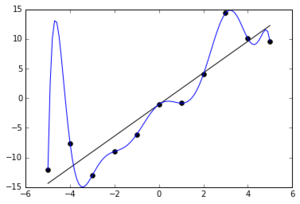
\includegraphics[width=0.5\linewidth]{"pictures/overfitted_data.png"}
	\caption{\textit{Noisy (roughly linear) data is fitted to a linear function and a polynomial function. Although the polynomial function is a perfect fit, the linear function can be expected to generalize better: if the two functions were used to extrapolate beyond the fitted data, the linear function should make better predictions.}}
	\label{fig:overfitting}
\end{figure}

\section{Linear regression}

\emph{Linear regression} \cite{linear_regression} is a statistical method used for predicting the value of a continuous outcome variable based on one or more input features. It models the relationship between the input features and the continuous outcome by fitting a linear function to observed data.

In the context of predicting time series, an input vector \(x_i\) is a subseries of data points of length \textit{seq\_len}, for which the output \(y_i\) is a prediction of the actual value of the data point following \(x_i\). Therefore, in the description below, the number of features of an input vector is \(d = \textit{seq\_len}\).

With that in mind, the general formulation of the linear regression model is as follows:

Given a set of \(n\) observations \(\{(x_i, y_i)\}_{i=1}^n\), where \(x_i \in \mathbb{R}^d\) represents the feature vector and \(y_i \in \mathbb{R}\) represents the continuous outcome, the linear regression model predicts the value of \(y\) as
\[
	\hat{y} = \beta_0 + \beta_1 x_{i,1} + \beta_2 x_{i,2} + \cdots + \beta_d x_{i,d},
\]
where \(\beta_0\) is the intercept term, and \(\beta_1, \beta_2, \ldots, \beta_d\) are the coefficients corresponding to the \(d\) features.

The model is trained to minimize the residual sum of squares (RSS), which measures the discrepancy between the observed values \(y_i\) and the predicted values \(\hat{y}_i\). The RSS is given by
\[
	RSS(\beta) = \sum_{i=1}^n (y_i - \hat{y}_i)^2 = \sum_{i=1}^n \left(y_i - (\beta_0 + \beta_1 x_{i,1} + \beta_2 x_{i,2} + \cdots + \beta_d x_{i,d})\right)^2,
\]
where \(n\) denotes the number of predicted values.

To find the optimal parameters \(\beta\), the RSS is minimized using analytical methods such as the normal equation or numerical optimization techniques such as gradient descent.






\section{Multilayer Perceptron}
The \emph{Multilayer Perceptron} (MLP) \cite{multilayer_perceptron} is a \emph{feedforward neural network}, that is made up of multiple layers of nodes in a directed graph, where each node from one layer is connected to all the nodes from the previous one.
MLPs are widely used in pattern recognition, classification, and regression problems due to their ability as networks to model complex nonlinear relationships in the input data.
An MLP consists of an input layer of neurons, one or more hidden layers, and an output layer.
Each node, except for those in the input layer, is a neuron that uses a nonlinear activation function to combine inputs from the previous layer and an additional \emph{bias term}.

\subsection{Structure of an MLP}

An MLP is made up of the following components:
\begin{itemize}
	\item \textbf{Input Layer:} The first layer of the network, which receives the input data to be processed. Each neuron in this layer represents a feature of the input data.
	\item \textbf{Hidden Layers:} One or more layers that perform computations on the inputs received and pass their output to the next layer. The neurons in these layers apply activation functions to their inputs to introduce nonlinearity.
	\item \textbf{Output Layer:} The final layer that produces the output of the network.
\end{itemize}

\subsection{Forward Propagation}

The process of computing the output of an MLP is called forward propagation.
In this process, the input data is passed through each layer of the network, transforming the data as it moves through. The output of each neuron is computed as follows:
\begin{equation}
	a^{(l)}_j = \phi\left(\sum_{i} w^{(l)}_{j,i} a^{(l-1)}_i + b^{(l)}_j\right),
\end{equation}
where
\begin{itemize}
	\item $a^{(l)}_j$ is the activation of the $j$-th neuron in the $l$-th layer;
	\item $\phi$ denotes the activation function, e.g. ReLU (\autoref{relu}), Softmax;
	\item $w^{(l)}_{j,i}$ represents the weight from the $i$-th neuron in the $(l-1)$-th layer to the $j$-th neuron in the $l$-th layer;
	\item $b^{(l)}_j$ is the bias term for the $j$-th neuron in the $l$-th layer;
	\item $a^{(l-1)}_i$ is the activation of the $i$-th neuron in the $(l-1)$-th layer.
\end{itemize}

\subsection{Backpropagation and Training}

To train an MLP, the backpropagation algorithm is used.
This algorithm adjusts the weights and biases of the network to minimize the difference between the actual output and the expected output.
The process involves computing the gradient of a \emph{loss function} with respect to each weight and bias in the network, and then using these gradients to update the weights and biases in the direction that minimizes the loss.
The loss function measures the error between the predicted output and the actual output. In our experiments, we used MSE as a loss function. The update rule for the weights is given by
\begin{equation}
	w^{(l)}_{j,i} \leftarrow w^{(l)}_{j,i} - \eta \frac{\partial \mathcal{L}}{\partial w^{(l)}_{j,i}},
\end{equation}
where
\begin{itemize}
	\item $\eta$ is the learning rate. If it is too small, the model will train very slowly and may get stuck in local minima. If it is too large, it might not converge.
	\item $\frac{\partial \mathcal{L}}{\partial w^{(l)}_{j,i}}$ is the partial derivative of the loss function $\mathcal{L}$ with respect to the weight $w^{(l)}_{j,i}$.
\end{itemize}
Similar updates are made for the biases.

Through iterative training involving forward propagation, loss calculation, and backpropagation, the MLP learns to approximate the function that maps data inputs to desired predictions.


\section{Convolutional neural network}
Convolutional Neural Networks (CNNs) \cite{convolutional_neural_network} are a class of deep neural networks, highly effective for analyzing visual imagery. They employ a mathematical operation called convolution, which allows them to efficiently process data in a grid-like topology, such as images.

\subsection{Architecture of Convolutional Neural Networks}
A typical CNN architecture comprises several layers that transform the input image to produce an output that represents the presence of specific features or class labels. The layers found in a CNN are:

\subsubsection{Convolutional Layer}
The convolutional layer applies a set of learnable filters to the input. Each filter activates specific features at certain spatial positions in the input. Mathematically, the convolution operation of each filter is defined as follows:
\[f(x, y) = (g * h)(x, y) = \sum_m\sum_n g(m,n) \cdot h(x-m, y-n),\]
where \(f(x, y)\) is the output, \(g\) is the filter, \(h\) is the input image, and \(*\) denotes the convolution operation. \(x\) and \(y\) range over output image dimensions; \(m\) and \(n\) range over the filter dimensions.

Following convolution, an \textbf{activation function} is applied to introduce nonlinearity into the model. The Rectified Linear Unit (ReLU) \label{relu} is commonly used:
\[\phi(x) = \max(0, x).\]

For time series forecasting, we use 1-dimensional convolutional neural network, which means that filter has \(1\) row.


\subsubsection{Pooling Layer}
The pooling layer reduces the spatial dimensions (width and height) of the input volume for the next convolutional layer.

\subsubsection{Fully Connected Layer}
Towards the end of the network, fully connected layers are used, where each input node is connected to each output by a learnable weight.

A simple diagram of the layers can be seen on figure \autoref{fig:cnn-diagram} (from \cite{cnn_diagram_source}). \footnote{In the image: the result of the convolution layer is a stack of output images, one for each filter.}

\begin{figure}[h!]
	\centering
	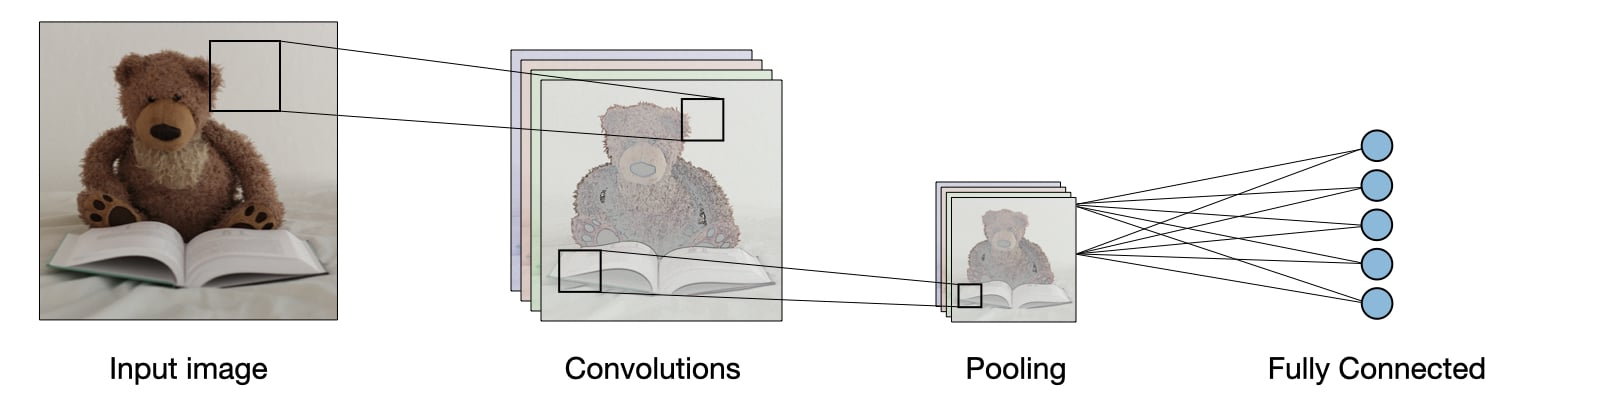
\includegraphics[width=0.5\linewidth]{"pictures/architecture-cnn-en.jpeg"}
	\caption{A simple diagram illustrating the different layers of the network working on an example input image.}
	\label{fig:cnn-diagram}

\end{figure}


\section{Residual Neural Network}


A Residual Neural Network (ResNet) is a type of deep learning model specifically designed to mitigate the vanishing gradient problem, where through backpropagation only the last few layers of the network get trained. ResNets introduce skip connections, also known as residual connections, which allow the input of a layer to be directly added to the output of a subsequent layer. This is mathematically expressed as
\[
	\mathbf{y} = \mathcal{F}(\mathbf{x}, \{W_i\}) + \mathbf{x},
\]
where $\mathbf{y}$ is the output of the layer, $\mathcal{F}$ represents the residual mapping to be learned by the layer, $\mathbf{x}$ is the input, and $\{W_i\}$ denote the weights of the layers.

The primary advantage of this architecture is its ability to facilitate the training of deeper networks by preserving the gradient flow through the network during backpropagation. This is achieved by allowing the backpropagation to bypass one or more layers, reducing the risk of gradient vanishing (where update gradients become exponentially small during backpropagation, slowing down training). As a result, ResNets can be trained to greater depths than CNNs, and can have more layers.


